\documentclass[a4papper, 11pt]{article}

\title{-- Digital Microelectronics --- SoundLoc -- \\ Localication of Soundsources by cross-correlating three $\Sigma\Delta$-microphon signals}
\author{Stefan Kull, Roy Seitz, Marco Zollinger}

\usepackage[T1]{fontenc}			%umlaute als eigene Zeichen
\usepackage[latin1]{inputenc}	%umlaute erkennen
\usepackage{lmodern}
\usepackage{amsmath} 					%mathematischen Textsatz.
\usepackage{amssymb}					%	-Erweiterte math. Sonderzeichen
\usepackage{dsfont}						%	-Mengen			
\usepackage[english]{babel}
\usepackage{textgreek}
\usepackage{siunitx}
\usepackage{graphicx}
\usepackage{caption}			%f�r \captionof

\usepackage[
	pdftitle={SoundLoc -- Digital Microelectronics Project},						%Titel des PDF Dokuments.
	pdfauthor={Stefan Kull, Roy Seitz, Marco Zollinger},									%Autor des PDF Dokuments.
	pdfsubject={Sound localication useing cross correlation of three microphones},		%Thema des PDF Dokuments.
	pdfcreator={LaTeX with hyperref and KOMA-Script},		%Erzeuger des PDF Dokuments.
	pdfkeywords={Cross correlatin, CIC, IP, AXI4\_Lite interface},						%auch f�r PDF Dokumente indexiert
	%	pdfpagemode=UseOutlines,								%Inhaltsverzeichnis anzeigen beim ffnen
	pdfdisplaydoctitle=true,								%Dokumenttitel statt Dateiname anzeigen.
	pdflang=en,												%Sprache des Dokuments.
	plainpages=false,
	hidelinks,												%keine Box um Links
	%	bookmarksopen.											%toc beim �ffnen expandiert
	pdfpagelabels
]{hyperref}

\usepackage[
%includeheadfoot,		%Kopf- und Fusszeilen verwenden
%headheight=15pt,		%H�he der Kopfzeile
left=30mm,				%abstand von Seitenraendern
right=30mm,				%
top=20mm,
bottom=20mm,
%			twoside
]{geometry}



\begin{document}
\maketitle
%\setcounter{tocdepth}{2}
%\tableofcontents

\section{Overview}
\label{sec:overview}

This Document describes the functionality and usage of the XCorr IP core.
It is supplied as a complete, ready to use IP core but without high level software support.
This is due to the project extent which is higher than expected.
Low level software access is provided but must be used carefully.
High level software support will be added in a future release.

The project Soundloc contains three microphones that deliver a $\Sigma\Delta$-modulated bitstream.
These are processed by another IP core SDM\_DECIMATOR, that delivers signed microphone data and an interrupt that indicates new values.

This IP core then calculates the cross-correlation between the three microphone signals and findes the Tau where the correlation is maximal.
To do this efficiently and in real-time, the correlation is calculated iteratively, using fast block RAM and DSP slices.
Detailed information to each stage is provided in the following sections.

\section{Parameter description}
\label{sec::parameters}

The IP core can be configured at compile time by several parameters, listed in table \ref{tbl::parameters}.
The number of stored samples is calculated according to (\ref{eq::parameter_sample_cnt}).
The calculated number of Taus is derived from (\ref{eq::parameter_tau_cnt}).
Tau ranges from Tau\textsubscript{min} to Tau\textsubscript{max}, given in (\ref{eq::parameter_tau_min}) and (\ref{eq::parameter_tau_max})

\begin{align}
	\text{N}_{\text{Sample}} &= 2^{\text{D\_SAMPLE\_ADDR\_WIDTH}}-1 \label{eq::parameter_sample_cnt} \\
	\text{N}_{\text{Tau}} &=2^{\text{D\_TAU\_ADDR\_WIDTH}}-2 \label{eq::parameter_tau_cnt} \\
	\text{Tau}_{\text{min}} &= -2^{\text{D\_TAU\_ADDR\_WIDTH} - 1}+1 \label{eq::parameter_tau_min} \\
	\text{Tau}_{\text{max}} &= 2^{\text{D\_TAU\_ADDR\_WIDTH} - 1}+1 \label{eq::parameter_tau_max}
\end{align}

\begin{table}[h]
	\centering
	\begin{tabular}{|l|c|c|l|l|}
		\hline 
		Parameter & Default & Range & Type & Description \\ 
		\hline 
		D\_WIDTH & 16 & 1\ldots18 & integer & Width of incoming microphone data\\
		\hline 
		D\_SAMPLE\_ADDR\_WIDTH & 10 & 7\ldots16 & integer & Address width for stored microphone samples\\
		\hline 
		D\_TAU\_ADDR\_WIDTH & 4 & 4\ldots6 & integer & Address width for calculated Taus \\
		\hline 
	\end{tabular} 
	\caption{Parameters for the XCorr}
	\label{tbl::parameters}
\end{table}

\section{Cross-correlation}
\label{sec::cic}

This section describes the calculation of the cross-correlation xcorr01 and xcorr02.
The first index indicates the reference microphone, which is fixed to mic0 (microphone 2 on PCB).
The correlation is recalculated each time a new value is available.
The recalculation takes N\textsubscript{Tau}$\,+\,5$ clock cycles.
An interrupt is asserted each time the cross-correlation has been recalculated.

\subsection{Implementation}

The cross-correlation of two discrete signals is defined per (\ref{eq::xcorr}).
Since only N\textsubscript{Sample} values are stored and available, the summation simplifies to (\ref{eq::xcorr_ptau}) for positive and  (\ref{eq::xcorr_ntau}) for negative Taus.

\begin{align}
\text{XCorr}_\text{ab}(\tau) &:= \sum_{n=-\infty}^{\infty}\text{a}\left[n\right]\text{b}\left[n+\tau\right] \label{eq::xcorr}\\
&= \sum_{n=0}^{\text{N}_\text{Sample}-\tau-2}\text{a}\left[n\right]\text{b}\left[n+\tau\right] \,\forall\,\tau\ge0 \label{eq::xcorr_ptau} \\
&= \sum_{n=0}^{\text{N}_\text{Sample}+\tau-2}\text{a}\left[n-\tau\right]\text{b}\left[n\right] \,\forall\,\tau<0 \label{eq::xcorr_ntau} \\	
\end{align}

Each time new data is available, all stored values are shifted by one storage position.
Therefore not the whole cross-correlation has to be calculated each time.
Only the newest value pair must be added and the oldest pair subtracted, resulting in two MAC-instructions per Tau and correlation.

\begin{figure}[htbp]
	\centering
	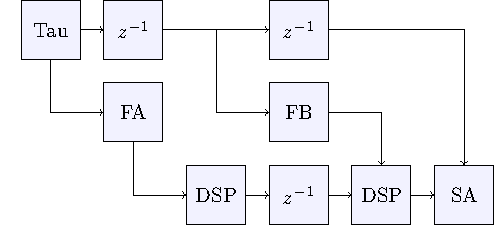
\includegraphics[scale = 1.5]{block_diagram/xcorr_diag.pdf}
	\captionof{figure}{Block diagram of pipelined calculation of cross-correlation}
	\label{fig::block_diag}
\end{figure}

To further improve performance, the calculation is pipelined.
Figure \ref{fig::block_diag} shows the data flow during recalculation.

\begin{itemize}
	\item Block Tau generates the actual Tau that is to be calculated.
	\item FA denotes fetch on RAM port A. It reads the corresponding cross-correlation and the (old) 	microphone values that are to multiply and subtract.	
	\item The first DSP performs $P = -(AB)+C$, with $A$ and $B$ connected to the microphone values from FA and $C$ to the cross-correlation value.
	\item FB fetches the (new) microphone values that are to multiply and add.
	\item The second DSP calculates $P = (AB)+C$, with the microphone values from FB and the prepared cross-correlation from the first DSP.
	\item Finally, SA denotes store on port A, which performs a write-back of the new calculated cross-correlation value.
\end{itemize}

Flip-flops are needed to store and shift the Taus corresponding to the single stages, as each block RAM fetch and store, as well as each MAC instruction needs one clock cycle.
Consequently the store command comes always three clock cycles after load.
Therefore neither collision nor simultaneous read / write is possible and no collision-detection is implemented.

Initially an internal variable is set to the minimal Value $-2^{31}$.
Each time a new Value is available at the output of the second DSP stage, these two values are compared.
If the new Value from the DSP is greater, the corresponding Tau is saved.
At the end of the recalculation, this tau is stored in the corresponding AXI register.
\section{Register description}
\label{sec::registers}
Three registers are present.
Register 0 is used to clear the internal RAM.
This starts an internal state machine that iterates over the whole RAM region.
While the internal RAM is being cleared, the whole block is locked and does not provide further functionality.
From register 1 and 2, the Taus corresponding to the maximal correlation value can be read.
Each register can be accessed directly by their address as described in section \ref{sec::driver}.

\begin{table}[h]
	\centering
	\begin{tabular}{|l|l|}
		\hline 
		Register Offset &  Description \\
		\hline 
		0x0	&  Write 1 to start clearing of internal RAM \\
		& Returns 1 if RAM is being cleared \\
		\hline 
		0x4	&  Tau for xcorr01\\
		\hline 
		0x8 & Tau for xcorr02 \\
		\hline
	\end{tabular} 
	\caption{Tau address}
	\label{tbl::tau_addr}
\end{table}

\section{Driver}
\label{sec::driver}

The IP core comes along with a driver to allow easy access by software.
There are two categories of functions, high and low level.
The usage of high level functions is recommended.
Care must be taken to not confuse the microphones. 
On the PCB they are numbered from 1 to 3 but in logic the numbering goes from 0 to 2.

\subsection{High level functions}
A typical use case with high level functions is as follows:
\begin{itemize}
	\item call XCORR\_Init(baseaddr, return\_imm) to initialize the IP core. \\
	This clears the internal RAM. If return\_imm is FALSE, the function will wait until the RAM is cleared, otherwise it will return immediately.\\
	Typically: XCORR\_Init(XCORR\_BASEADDR, 0).
	\item Call XCORR\_GetTau(baseaddr, \&tau01, \&tau02). \\
	This stores the taus in the provided variables tau01 and tau02.
\end{itemize}


\subsection{Low level functions}
The core can also be used by addressing the registers directly.
For this purpose two low-level functions are available.
These functions are implemented as macros and should only be used if really necessary.

\begin{itemize}
	\item XCORR\_mWriteReg(BaseAddress, RegOffset, Data) \\
		Write data to the specified Register. 
	\item XCORR\_mReadReg(BaseAddress, RegOffset) \\		
		Read the content of the specified register.
\end{itemize}

\section{Test and verification}
\label{sec::test}

The core can easily be simulated by using the AXI traffic generator IP from Xilinx and feeding some well known values to the inputs.
No additional simulation files are available.
Software verification is not supported.

\section{Compatibility and License}
The core is tested under Vivado version 2016.2 and on Artix7 and Zynq7 FPGA.
The core does use hardware specific resources.
It is therefore not guaranteed to run on other FPGAs.
Since only 4 DSP slices and block RAM is used, it should run on nearly every FPGA with enough block RAM available.
However, this is not tested and may require changes to the core hdl files.
The core is supplied under no license or copyright but is the intellectual property of the authors.

\end{document}